\documentclass[12pt]{article}
% Chinese Support
\usepackage{xeCJK}
\setCJKmainfont{STSong}
% \setmainfont{Times New Roman}

\usepackage{float}

% for symbol
\usepackage{gensymb}
% matrix
\usepackage{amsmath}

% For images
\usepackage{graphicx}
\graphicspath{ {./screenshoot/} }

\newcommand{\numpy}{{\tt numpy}}    % tt font for numpy

\topmargin -1.in
\textheight 9in
\oddsidemargin -.25in
\evensidemargin -.25in
\textwidth 7in


\usepackage{listings}
\usepackage{color}
\usepackage{xcolor}

\definecolor{dkgreen}{rgb}{0,0.6,0}
\definecolor{gray}{rgb}{0.5,0.5,0.5}
\definecolor{mauve}{rgb}{0.58,0,0.82}
\definecolor{textblue}{rgb}{.2,.2,.7}
\definecolor{textred}{rgb}{0.77,0,0}
\definecolor{textgreen}{rgb}{0,0.43,0}

% \setmonofont{FiraCode-Regular}
\lstset{frame=tb,
  language=C++,
  aboveskip=3mm,
  belowskip=3mm,
  showstringspaces=false,
  columns=flexible,
  basicstyle={\ttfamily},
  numbers=none,
  numberstyle=\tiny\color{gray},
  keywordstyle=\color{blue}\itshape,
  stringstyle=\color{mauve},
  breaklines=true,
  breakatwhitespace=true,
  commentstyle=\color{textred}\itshape,
  tabsize=3
}



% Content start below
\begin{document}

\author{陈铭涛\\16340024}
\title{计算机图形学 Homework 6 - Lights and Shading}
% \date{\vspace{-5ex}}
\maketitle

\medskip

% ========== Begin answering questions here

\section{Basic}

\begin{enumerate}
    \item 实现Phong光照模型:
    \begin{description}
        \item[$\bullet$ ]场景中绘制一个cube
        \item[$\bullet$ ]自己写shader实现两种shading: Phong Shading 和 Gouraud Shading,并解释两种shading的实现原理
        \item[$\bullet$ ]合理设置视点、光照位置、光照颜色等参数,使光照效果明显显示 
    \end{description}
    Cube 的实现方法与前两次作业相近,在本次作业中实现了\lstinline{LightingCube}类,其中包含了 Phong 着色器和 Gouraud 着色器。
    
    Phong 着色法和 Gouraud 着色法都是由环境光照、漫反射光照和镜面光照组合而成的,着色器中除接收变换矩阵外的变量,还接收如下与光照相关的变量:
    \begin{lstlisting}
uniform vec3 lightPos;
uniform vec3 lightColor;
uniform vec3 objectColor;
uniform vec3 viewPos;
uniform float ambientStrength;
uniform float specularStrength;
uniform float diffuseStrength;
uniform int shininess;
    \end{lstlisting}
    其中\lstinline{lightPos}为光源的位置,\lstinline{lightColor}为光照的颜色,\lstinline{objectColor} 为物体的颜色,
    \lstinline{viewPos}为摄像机的位置,\lstinline{ambientStrength}为环境光照因子,\lstinline{diffuseStrength}为漫反射因子,
    \\\lstinline{specularStrength} 为镜面光照因子,\lstinline{shininess}为镜面的反光度。

    顶点着色器需要输入顶点的法向量数据:
    \begin{lstlisting}
layout (location = 1) in vec3 aNormal;
    \end{lstlisting}
    
    Phong着色法的原理是根据物体顶点法向量,对表面各个像素进行双线性插值,决定像素的颜色。
    而 Gouraud 着色法则根据物体顶点的法向量对顶点的颜色采用 Phong 模型进行插值,片段着色器填充像素的颜色时则仅根据顶点的颜色和距离进行插值填充。

    由于法向量是一个方向向量,当应用了不等比缩放时会导致其在世界坐标中效果不正确,解决的方法是使用法线矩阵乘以原法向量来消除影响,法线矩阵为:
    \begin{equation}
        \label{normal}
        N = (M^{-1})^T
    \end{equation}
    其中 M 为模型矩阵。

    Phong 着色法与 Gouraud 着色法相比,真实度更高,镜面反射的效果更加准确,但是需要对每个像素点进行计算,所需的计算量更大。

    Gouraud 着色法在渲染与位置相关度较大的光照效果时效果不佳,比如当镜面光照的高光位于顶点上时,Gouraud 着色法会使高光在表面不自然地扩散。
    如Figure1,2:

    \begin{figure}[H]
        \centering
        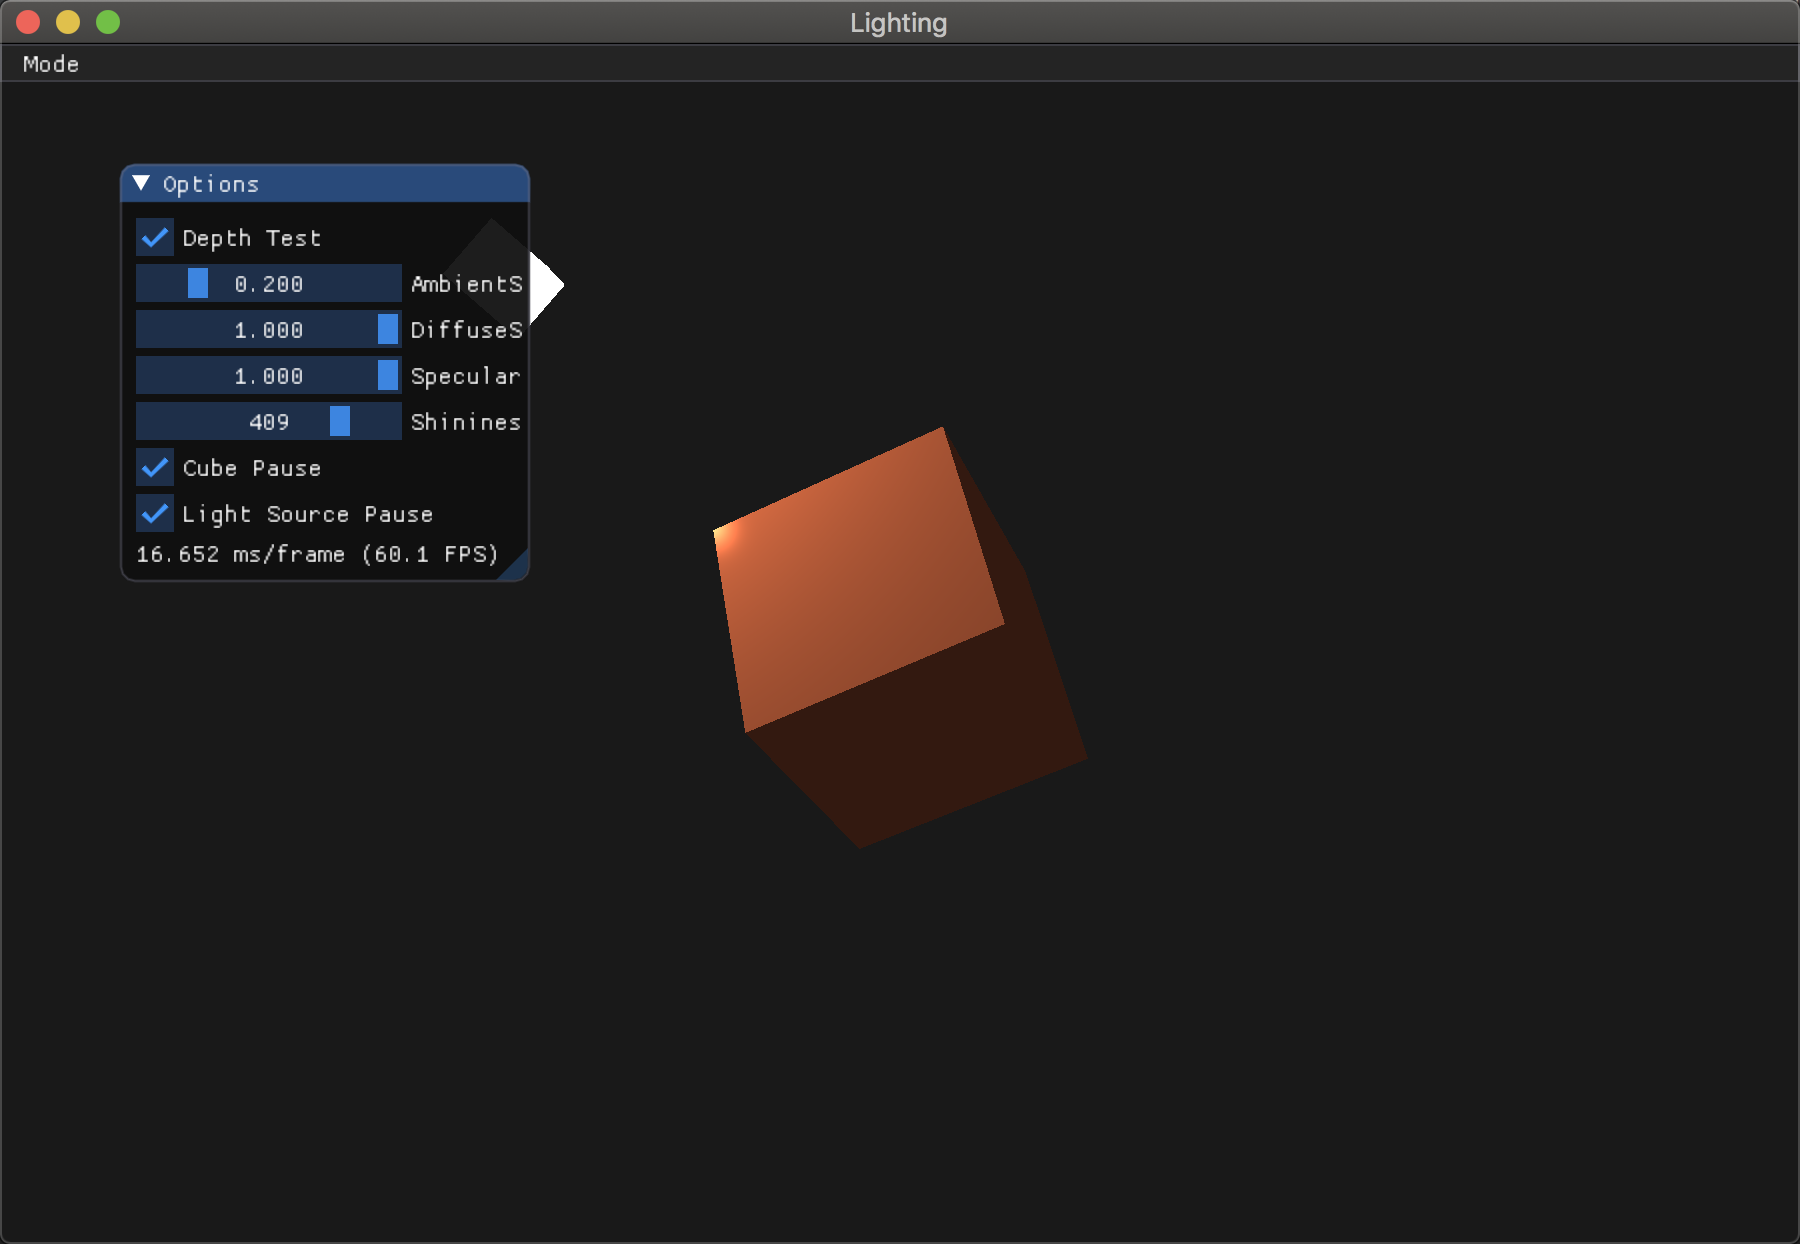
\includegraphics[scale=0.3]{phong1.png}
        \caption{Phong着色法,高光位于顶点上}
        \label{fig: phong1}
    \end{figure}

    \begin{figure}[H]
        \centering
        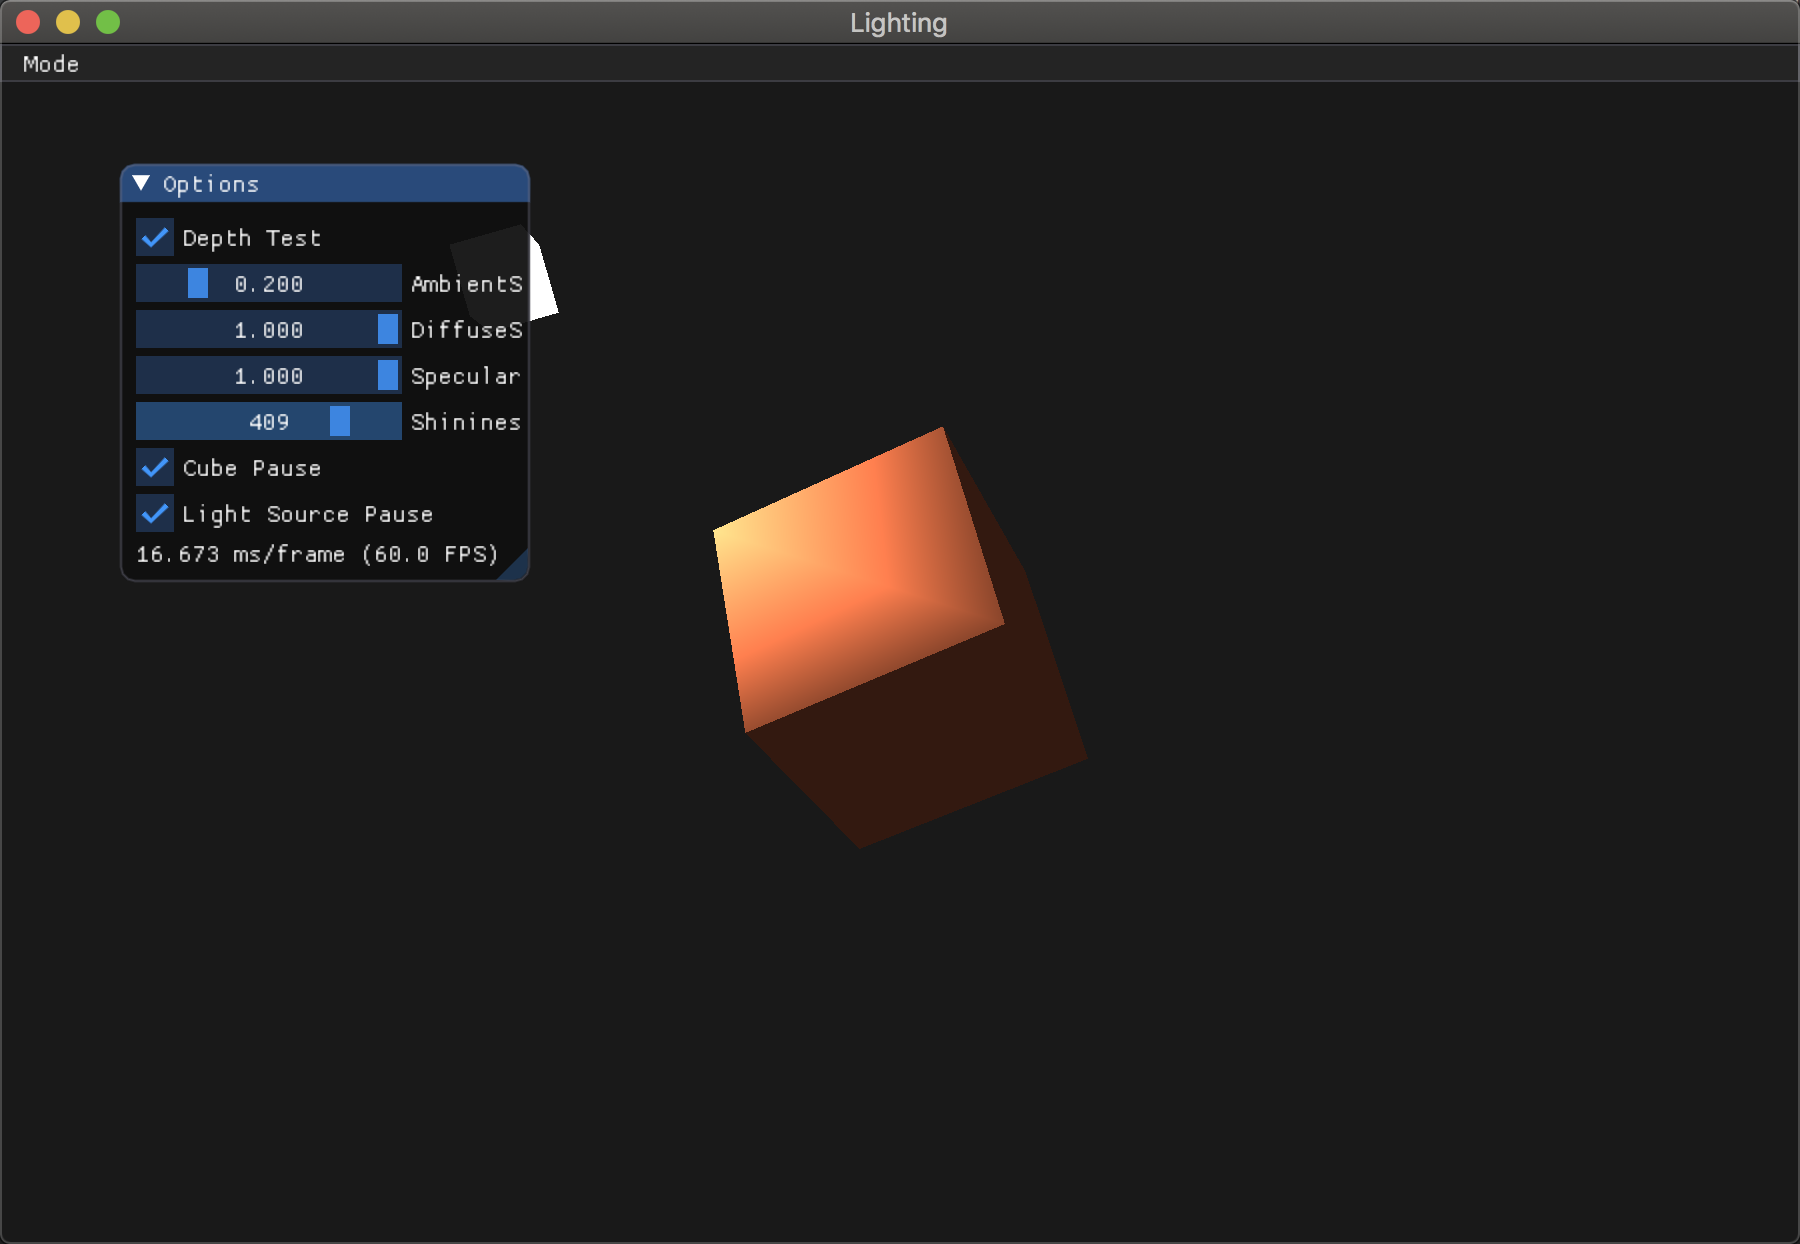
\includegraphics[scale=0.3]{gouraud1.png}
        \caption{Gouraud着色法,高光位于顶点上}
        \label{fig: phong1}
    \end{figure}

    当高光不扩散到任何顶点上时,Gouraud 着色法将不会渲染出其效果,如Figure3,4:
        
    \begin{figure}[H]
        \centering
        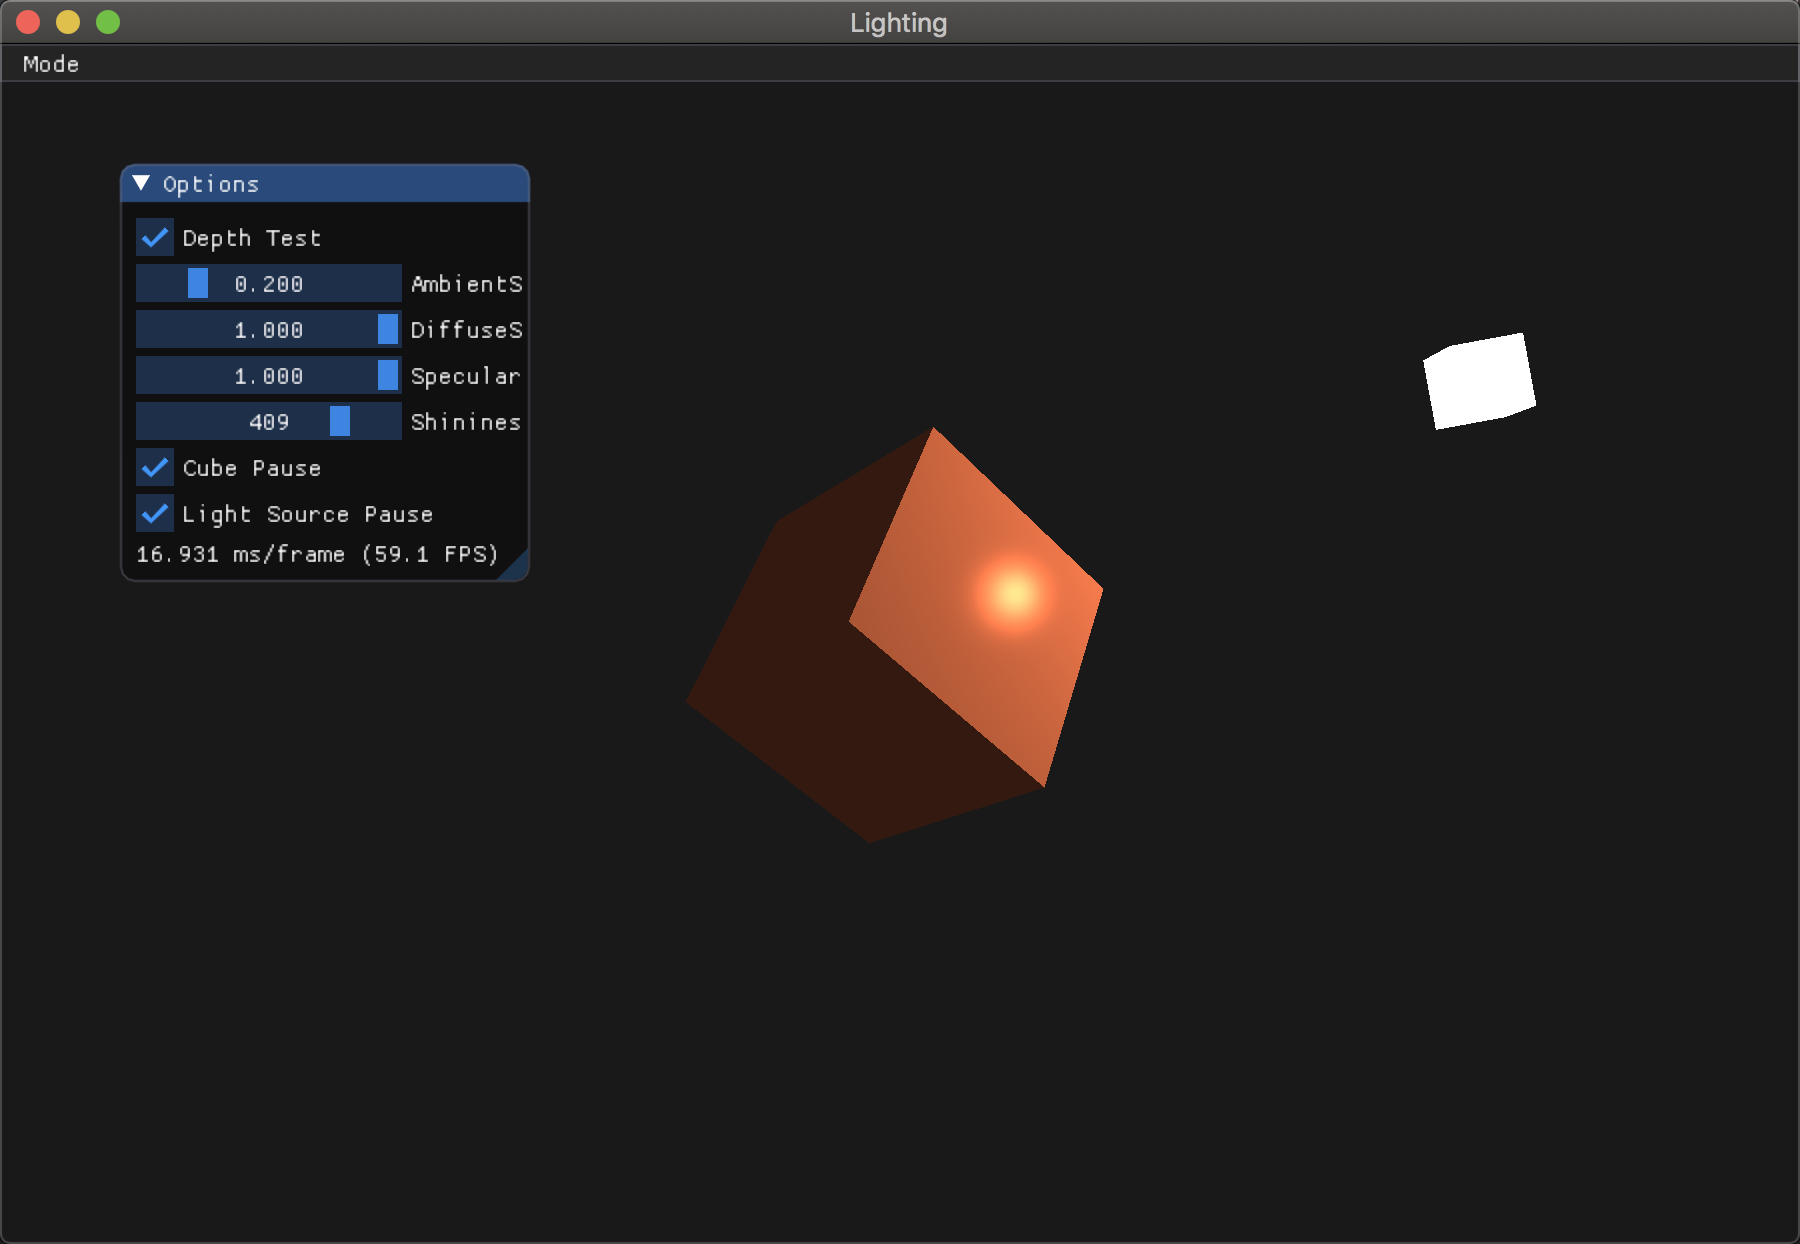
\includegraphics[scale=0.35]{phong2.png}
        \caption{Phong着色法,高光不位于任何顶点上}
        \label{fig: phong2}
    \end{figure}

    \begin{figure}[H]
        \centering
        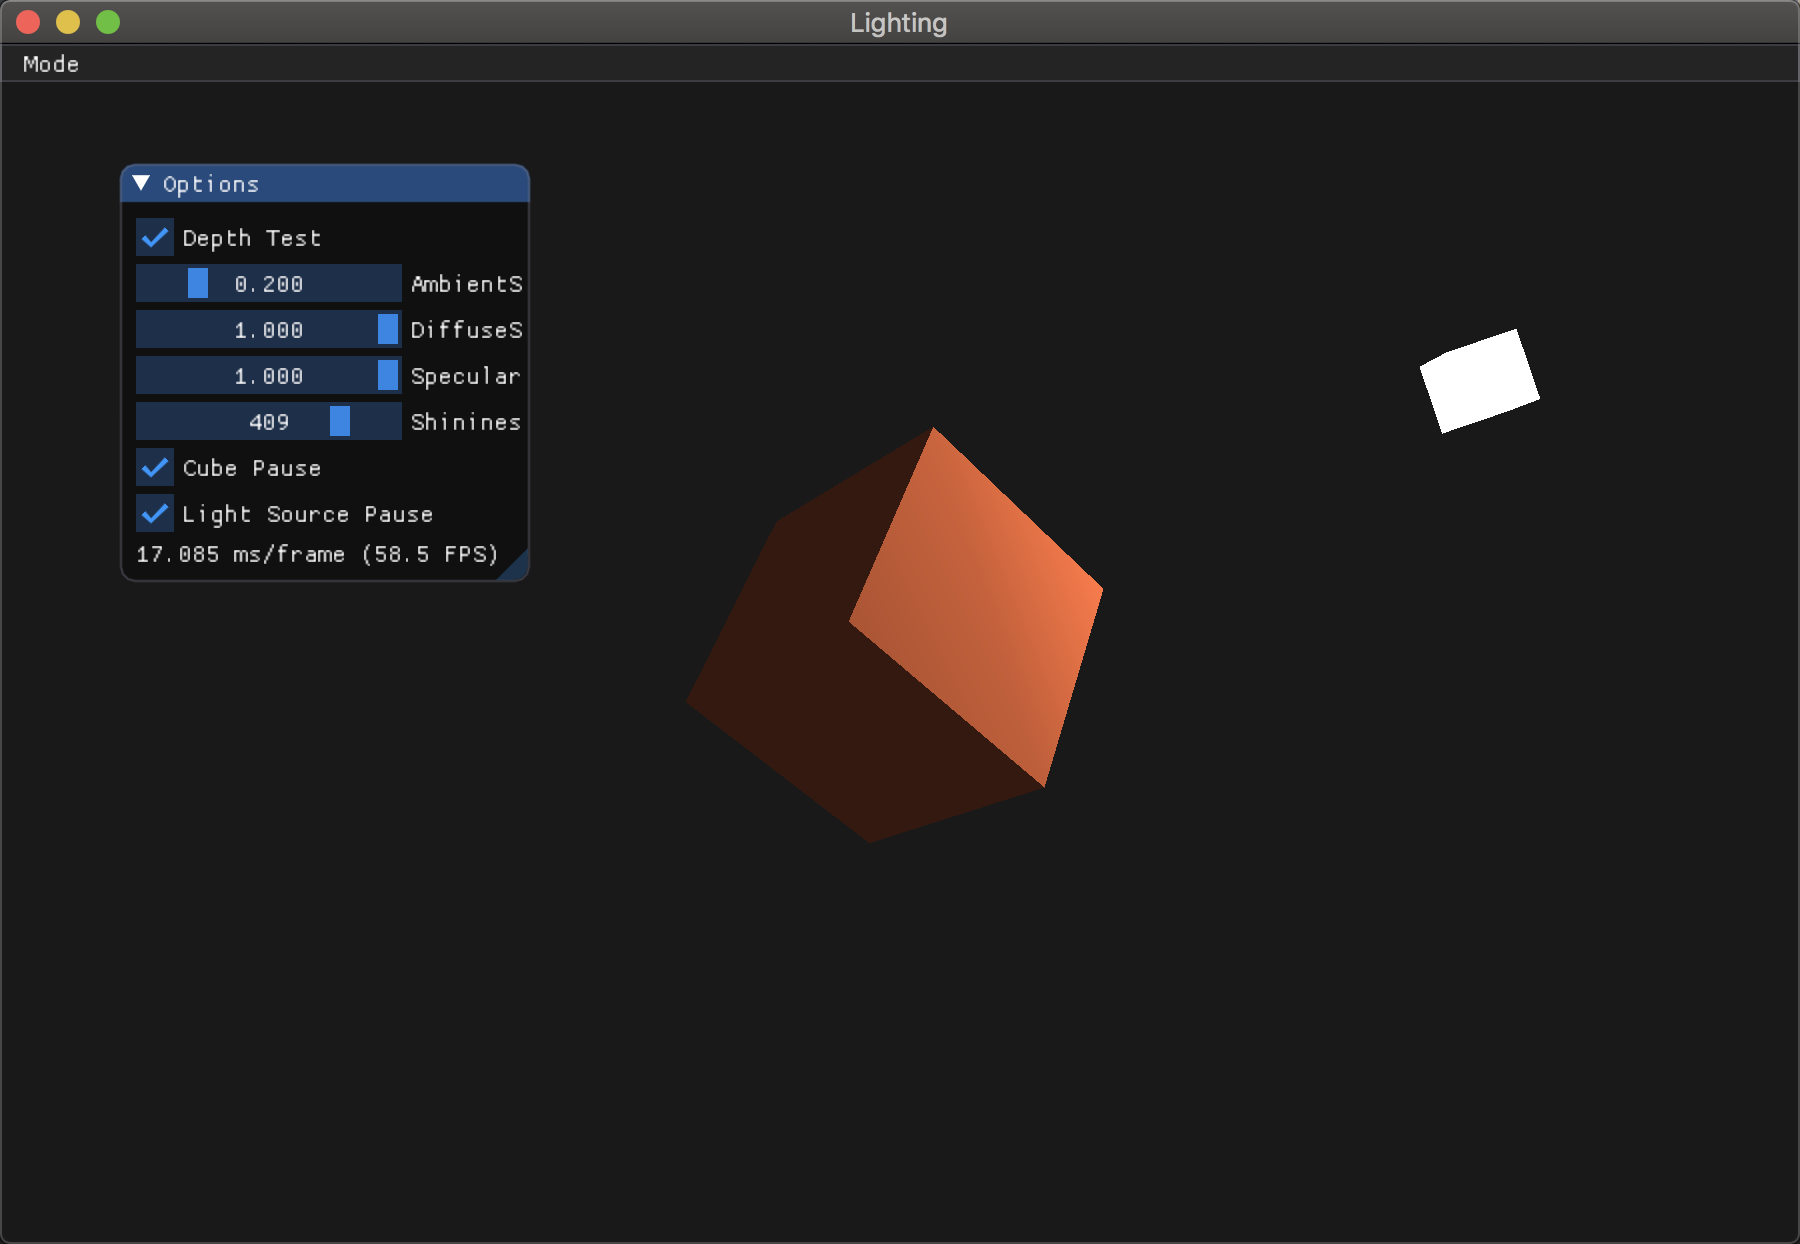
\includegraphics[scale=0.35]{gouraud2.png}
        \caption{Gouraud着色法,高光不位于任何顶点上}
        \label{fig: phong2}
    \end{figure}

    \item 使用GUI,使参数可调节,效果实时更改:
    \begin{description}
        \item[$\bullet$ ]GUI里可以切换两种shading
        \item[$\bullet$ ]使用如进度条这样的控件,使ambient因子、diffuse因子、specular因子、反光度等参数可调节,光照效果实时更改
    \end{description}

    使用 GUI 在右上角添加了用于切换着色方法的菜单,并添加了可以调节ambient, diffuse 以及 specular 因子和反光度参数的滑块,效果如图:
    \begin{figure}[!htb]
        \centering
        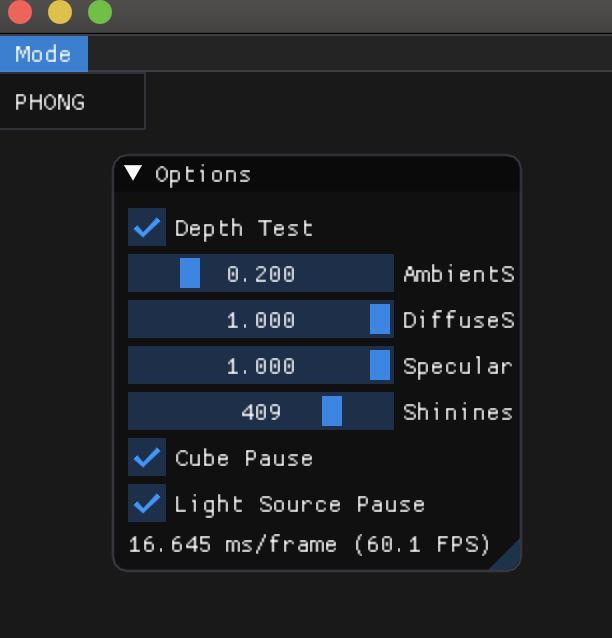
\includegraphics[scale=0.8]{GUI.png}
        \caption{GUI}
        \label{fig: gui}
    \end{figure}
\end{enumerate}

\section{ Bonus }
\begin{enumerate}
    \item 当前光源为静止状态,尝试使光源在场景中来回移动,光照效果实时更改。
    
    采用了在先前作业中实现的椭圆运动变换使光源在场景中可以椭圆形绕物体移动,将光源用一个纯白的立方体表示,每次在循环中获取立方体所处的位置作为光源坐标。
    
    物体自身也以一定的速度进行自转,在 GUI 中对光源的运动和物体自转提供了暂停的选项,方便寻找某一特定角度进行截图。

    具体动态效果请见 demo 视频。
\end{enumerate}

\end{document}
\grid
\grid
